\chapter{Agenti basati su conoscenza}

Abbiamo trattato:
\begin{itemize}
	\item Agenti con stato e con obiettivo in mondi osservabili con stati atomici e azioni descrivibili in maniera semplice; enfasi sul processo di ricerca.
	\item Descrizioni ``fattorizzate'' (come nei CSP) che consentono di iniziare a ``guardare dentro'' lo stato,
	      descritto come un insieme di caratteristiche rilevanti (o \textbf{\textit{feature}}).
\end{itemize}
Vogliamo adesso migliorare le \textbf{capacità di ragionamento} dei nostri agenti dotandoli di rappresentazioni di mondi più complessi e \textbf{astratti}, non descrivibili semplicemente:\ agenti \textbf{\textit{basati su conoscenza}}, dotati di una KB (\textit{Knowledge Base}) con conoscenza espressa in maniera esplicita e dichiarativa.

\begin{figure}[H]
	\centering
	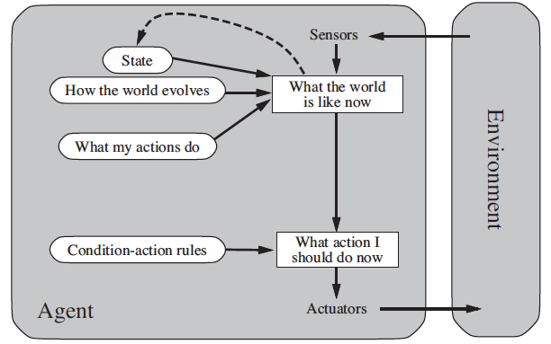
\includegraphics[width=0.7\textwidth]{immagini/AgentiConoscenti.png}
	\caption*{Agenti basati su modello}
\end{figure}

\subsubsection{Agenti ``Knowledge Based''}

La maggior parte dei problemi di I.A. sono ``\textit{knowledge intensive}''.\
Il mondo è tipicamente complesso:\ ci serve una rappresentazione \textbf{\textit{parziale}} e \textbf{\textit{incompleta}} (un'astrazione) del mondo utile agli scopi dell'agente.\

Per ambienti parzialmente osservabili e complessi ci servono linguaggi di rappresentazione della conoscenza più espressivi e capacità inferenziali.\
La conoscenza può essere codificata a mano ma anche estratta dai testi o appresa dall'esperienza.

\subsubsection{Approccio dichiarativo vs procedurale}

La KB racchiude tutta la conoscenza necessaria a decidere l'azione da compiere in forma \textbf{\textit{dichiarativa}}.\
L'alternativa (\textit{approccio procedurale}) è scrivere un programma che implementa il processo decisionale, una volta per tutte.

Un agente KB è più flessibile:\ più semplice acquisire conoscenza incrementalmente e modificare il comportamento con l'esperienza.

\section{Agente basato su conoscenza}

Un agente basato su conoscenza mantiene una \textbf{\textit{base di conoscenza}} (KB):\ un insieme di enunciati espressi in un linguaggio di rappresentazione.\
Interagisce con la KB mediante una interfaccia funzionale \textit{Tell-Ask}:
\begin{itemize}
	\item \textit{Tell}:\ per aggiungere nuovi enunciati a KB
	\item \textit{Ask}:\ per interrogare la KB
	\item \textit{Retract}:\ per eliminare enunciati
\end{itemize}
Gli enunciati nella KB rappresentano le \textbf{opinioni}{\slash}\textbf{credenze dell'agente}.\
Le risposte $\alpha$ devono essere tali che $\alpha$ è una conseguenza (discende necessariamente) della KB.\

\textit{Il problema}:\ data una base di conoscenza KB, contenente una rappresentazione dei fatti che si \textbf{ritengono veri}, vorrei sapere se un certo fatto $\alpha$ è vero di conseguenza
\[\mathrm{KB} \models \alpha\quad (\mathit{conseguenza\ logica})\]

\subsubsection{Base di conoscenza vs base di dati}

\textit{Base di conoscenza}:\ una rappresentazione esplicita, parziale e compatta, in un linguaggio simbolico, che contiene fatti di tipo specifico e fatti di tipo generale, o regole.\

\noindent\textit{Base di dati}:\ solo fatti specifici, solo recupero.\

Quello che caratterizza una KB è la \textbf{\textit{capacità inferenziale}}, cioè la capacità di derivare nuovi fatti da quelli memorizzati esplicitamente.\

\subsubsection{Il trade-off fondamentale della R.C.}
Sfortunatamente più il linguaggio è \textit{espressivo}, meno \textit{efficiente} è il meccanismo inferenziale.\
Il problema ``fondamentale'' nella rappresentazione della conoscenza (R.C.) è trovare il giusto compromesso tra:\ espressività del linguaggio di rappresentazione e complessità del meccanismo inferenziale.\
Questi due obiettivi sono in contrasto e si tratta di mediare tra queste due esigenze.

\subsection{Formalismi per la R.C.}

Un formalismo per la rappresentazione della conoscenza ha tre componenti:
\begin{enumerate}
	\item Una \textbf{\textit{sintassi}}:\ un linguaggio composto da un vocabolario e regole per la formazione delle frasi (\textit{enunciati}).
	\item Una \textbf{\textit{semantica}} che stabilisce una corrispondenza tra gli enunciati e fatti del mondo; se un agente ha un enunciato $\alpha$ nella sua KB, crede che il fatto corrispondente sia vero nel mondo.
	\item Un \textbf{\textit{meccanismo inferenziale}} (codificato, o meno, tramite regole di inferenza come nella logica) che ci consente di inferire nuovi fatti.
\end{enumerate}

\subsubsection{Logica come linguaggio per la R.C.}

Qual è la complessità computazionale del problema KB $\models \alpha$ nei vari linguaggi logici?\
Quali sono gli algoritmi di decisione e le strategie di ottimizzazione?\
I linguaggi logici come calcolo proposizionale (PROP) e logica dei predicati (FOL) sono adatti per la rappresentazione della conoscenza?

\section{Agenti logici:\ calcolo proposizionale}

\subsubsection{Sintassi}

La sintassi definisce quali sono le frasi legittime (\textbf{ben formate}) del linguaggio:

\begin{table}[H]
	\centering
	\begin{tabular}{l l p{16em}}
		\textit{formula}          & $\rightarrow$ & \textit{formulaAtomica} $|$ \textit{formulaComplessa}                        \\
		\textit{formulaAtomica}   & $\rightarrow$ & \textbf{\textit{True}} $|$ \textbf{\textit{False} }$|$ \textit{simbolo}      \\
		\textit{simbolo}          & $\rightarrow$ & \textbf{\textit{P}} $|$\textbf{\textit{Q}} $|$ \textbf{\textit{R}} $|$ \dots \\
		\textit{formulaComplessa} & $\rightarrow$ & $\lnot formula$                                                              \\
		                          &               & $|$ $(formula\ \land\ formula)$                                              \\
		                          &               & $|$ $(formula\ \lor\ formula)$                                               \\
		                          &               & $|$ $(formula\ \Rightarrow\ formula)$                                        \\
		                          &               & $|$ $(formula\ \Leftrightarrow\ formula)$                                    \\
	\end{tabular}
\end{table}

\noindent Esempio:\ $((\mathrm{A} \land \mathrm{B}) \Rightarrow \mathrm{C})$

\noindent Possiamo omettere le parentesi assumendo questa \textbf{precedenza} tra gli operatori:
\[
	\lnot\ >\ \land\ >\ \lor\ >\ \Rightarrow\ >\ \Leftrightarrow
\]

\subsubsection{Semantica e mondi possibili (modelli)}

La semantica ha a che fare col significato delle frasi:\ definisce se un enunciato è vero o falso rispetto ad una \textbf{\textit{interpretazione}} (mondo possibile).\
Un'interpretazione definisce un valore di verità per tutti i simboli proposizionali.\

\vspace{12pt}
Per esempio:\ $\{\mathrm{P}_{1,1}\ \mathit{vero},\ \mathrm{P}_{1,2}\ \mathit{falso},\ \mathrm{W}_{2,3}\ \mathit{vero}\}$

\vspace{12pt}

\noindent Il valore di una formula complessa è fissato di conseguenza:
\[\mathrm{P}_{1,1} \Rightarrow \mathrm{W}_{2,3} \lor \mathrm{P}_{1,2}\ \grave{e}\ \mathrm{vera\ in\ questa\ interpretazione}.\]
Un \textbf{\textit{modello}} è un'interpretazione che \textit{rende vera} una formula o un insieme di formule.\

\subsubsection{Semantica composizionale}
Il significato di una frase è determinato dal significato dei suoi componenti, a partire dalle frasi atomiche (i simboli proposizionali).\
\begin{itemize}
	\item \textit{True} sempre vero; \textit{False} sempre falso
	\item P $\land$ Q, vero se P e Q sono veri
	\item P $\lor$ Q, vero se P oppure Q, o entrambi, sono veri
	\item $\lnot$P  vero se P è falso
	\item P $ \Rightarrow$ Q, vero se P è falso oppure Q è vero
	\item P $ \Leftrightarrow$ Q,  vero se entrambi veri o entrambi falsi
\end{itemize}

\subsubsection{Conseguenza logica}

Una formula $\alpha$ è \textbf{\textit{conseguenza logica}} di un insieme di formule KB se e solo se in ogni modello di KB, anche $\alpha$ è vera (KB $\models \alpha$).\
Indicando con $M(\alpha)$ l'insieme delle interpretazioni che rendono $\alpha$ vera (i \textbf{modelli} di $\alpha$) e con \textit{M}(KB) i modelli dell'insieme di formule in KB\dots
\[
	\mathrm{KB} \models \alpha\  sse\  M(\mathrm{KB}) \subseteq M(\alpha)
\]

\subsubsection{Equivalenza logica:\ leggi}

\textbf{Equivalenza logica}:\ A $\equiv$ B se e solo se A $\models$ B e B $\models$ A.

\begin{table}[H]
	\centering
	\begin{tabular}{r c l}
		$(\alpha\ \land\ \beta)$                  & $\equiv$ & $(\beta\ \land\ \alpha)$ \quad commutatività di $\land$                                             \\
		$(\alpha\ \lor\ \beta)$                   & $\equiv$ & $(\beta\ \lor\ \alpha)$ \quad commutatività di $\lor$                                               \\
		$((\alpha\ \land\ \beta)\ \land\ \gamma)$ & $\equiv$ & $(\alpha\ \land\ (\beta\ \land\ \gamma))$ \quad associatività di $\land$                            \\
		$((\alpha\ \lor\ \beta)\ \lor\ \gamma)$   & $\equiv$ & $(\alpha\ \lor\ (\beta\ \lor\ \gamma))$ \quad associatività di $\lor$                               \\
		$\lnot(\lnot\alpha)$                      & $\equiv$ & $\alpha$ \quad doppia negazione                                                                     \\
		$(\alpha\ \Rightarrow\ \beta)$            & $\equiv$ & $(\lnot \beta\ \Rightarrow\ \lnot \alpha)$ \quad contrapposizione                                   \\
		$(\alpha\ \Rightarrow\ \beta)$            & $\equiv$ & $(\lnot \alpha\ \lor\ \beta)$ \quad eliminazione dell'implicazione                                  \\
		$(\alpha\ \Leftrightarrow\ \beta)$        & $\equiv$ & $(\alpha\ \Rightarrow\ \beta)\ \land\ (\beta\ \Rightarrow\ \alpha)$ \quad eliminazione del sse      \\
		$\lnot(\alpha\ \land\ \beta)$             & $\equiv$ & $(\lnot \alpha\ \lor\ \lnot \beta)$ \quad De Morgan                                                 \\
		$\lnot(\alpha\ \lor\ \beta)$              & $\equiv$ & $(\lnot \alpha\ \land\ \lnot \beta)$ \quad De Morgan                                                \\
		$(\alpha\ \land\ (\beta\ \lor\ \gamma))$  & $\equiv$ & $((\alpha\ \land\ \beta\ )\ \lor\ (\alpha \land \gamma))$ \quad distributività di $\land$ su $\lor$ \\
		$(\alpha\ \lor\ (\beta\ \land\ \gamma))$  & $\equiv$ & $((\alpha\ \lor\ \beta\ )\ \land\ (\alpha \lor \gamma))$ \quad distributività di $\lor$ su $\land$  \\
	\end{tabular}
\end{table}

\subsubsection{Validità, soddisfacibilità}

A è \textbf{valida} \textit{sse} è vera in tutte le interpretazioni (anche detta tautologia).

\noindent A è \textbf{soddisfacibile} \textit{sse} esiste un'interpretazione in cui A è vera.\

Ne discende che
\begin{center}
	A è valida sse $\lnot$A è insoddisfacibile
\end{center}

\subsubsection{Inferenza per calcolo proposizionale}

\begin{itemize}
	\item \textit{Model checking}:\ una forma di inferenza che fa riferimento alla definizione di conseguenza logica (si enumerano i possibili modelli), per esempio usando la tecnica delle tabelle di verità.\
	\item Algoritmi per la \textit{soddisfacibilità} (SAT):\ KB $\models$ A \textit{sse} (KB $\land\ \lnot$A) è insoddisfacibile.\ Un problema può essere ricondotto all'altro.
\end{itemize}

\subsection{L'algoritmo TT-entails}
\[\mathrm{KB} \models\alpha?\]
Enumera tutte le possibili interpretazioni di KB (\textit{k simboli}, $2^k$ possibili interpretazioni).\
Per ciascuna interpretazione
\begin{itemize}
	\item Se non soddisfa KB, OK.
	\item Se soddisfa KB, si controlla che soddisfi anche $\alpha$.
\end{itemize}
Se si trova anche solo un'interpretazione che soddisfa KB e non $\alpha$ la risposta sarà NO.

\begin{figure}[H]
	\centering
	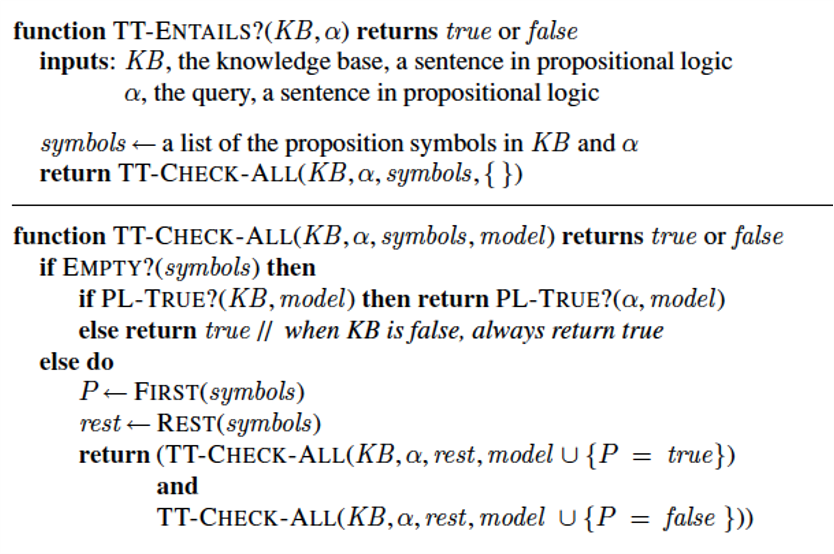
\includegraphics[width=0.8\textwidth]{immagini/TTEntails.png}
\end{figure}

\subsection{Algoritmi per la soddisfacibilità (SAT)}

Usano KB in \textbf{forma a clausole} (insiemi di letterali)
\[\{\mathrm{A},\ \mathrm{B}\}\ \{\lnot \mathrm{B},\ \mathrm{C},\ \mathrm{D}\}\ \{\lnot \mathrm{A},\ \mathrm{F}\}\]
La forma a clausole è la forma normale congiuntiva (CNF):\ una congiunzione di disgiunzioni di letterali
\[(\mathrm{A} \lor \mathrm{B})\ \land\ (\lnot \mathrm{B} \lor \mathrm{C} \lor \mathrm{D}) \land (\lnot \mathrm{A}  \lor \mathrm{F})\]
Non è restrittiva:\ è sempre possibile ottenerla con trasformazioni che preservano l'equivalenza logica.\

\subsubsection{Trasformazione in forma a clausole}
I passi sono:
\begin{enumerate}
	\item Eliminazione del $\Leftrightarrow$: (A $\Leftrightarrow$ B) $\equiv$ (A $\Rightarrow$ B) $\land$ (B $\Rightarrow$ A)
	\item Eliminazione dell' $\Rightarrow$: (A $\Rightarrow$ B) $\equiv$ ($\lnot$A $\lor$ B)
	\item Negazioni all'interno:
	      \begin{table}[H]
		      \centering
		      \begin{tabular}{l l}
			      $\lnot$(A $\lor$ B) $\equiv$ ($\lnot$A $\land$ $\lnot$B) & (De Morgan) \\
			      $\lnot$(A $\land$ B) $\equiv$ ($\lnot$A $\lor$ $\lnot$B) &             \\
		      \end{tabular}
	      \end{table}
	\item Distribuzione di $\lor$ su $\land$:\ 	(A $\lor$ (B $\land$ C)) $\equiv$ (A $\lor$ B) $\land$ (A $\lor$ C)
\end{enumerate}

\subsection{L'algoritmo DPLL per la soddisfacibilità}

DPLL:\ Davis, Putman, e poi Lovemann, Loveland

Parte da una KB in \textbf{forma a clausole}.\
È un'enumerazione \textit{in profondità} di tutte le possibili interpretazioni alla ricerca di un modello.\
Tre miglioramenti rispetto a TTEntails:
\begin{enumerate}
	\item terminazione anticipata,
	\item euristica dei simboli (o letterali) puri,
	\item euristica delle clausole unitarie.
\end{enumerate}

\subsubsection{Terminazione anticipata}

Si può decidere sulla verità di una clausola anche con interpretazioni parziali:\ basta che un \textit{letterale} sia vero.\ Per esempio se A è vero, lo sono anche \{A, B\} e \{A, C\} indipendentemente dai valori di B e C.\

Se anche una sola clausola è falsa l'interpretazione non può essere un modello dell'insieme di clausole.\

\subsubsection{Simboli puri}

\textit{Simbolo puro}:\ un simbolo che appare con lo stesso segno in tutte le clausole, per esempio
\[ \{\mathrm{A}, \lnot \mathrm{B}\}\ \{\lnot \mathrm{B}, \lnot \mathrm{C}\}\ \{\mathrm{C}, \mathrm{A}\} \quad \mathrm{A\ puro,\ B\ anche}\]
Nel determinare se un simbolo è puro se ne possono trascurare le occorrenze in clausole già rese vere.\

I simboli puri possono essere assegnati a \textit{True} se il letterale è positivo, \textit{False} se negativo.\
Non si eliminano modelli utili:\ se le clausole hanno un modello continuano ad averlo dopo questo assegnamento.\ L'assegnamento è obbligato.

\subsubsection{Clausole unitarie}

\textit{Clausola unitaria}:\ una clausola con un solo letterale \textbf{\textit{non assegnato}}.\ Per esempio \{B\} è unitaria ma anche \{B, $\lnot$C\} è unitaria quando C = \textit{True}.

Conviene assegnare prima valori al letterale in clausole unitarie.\ L'assegnamento è univoco (\textit{True} se positivo, \textit{False} se negativo).
\begin{figure}[H]
	\centering
	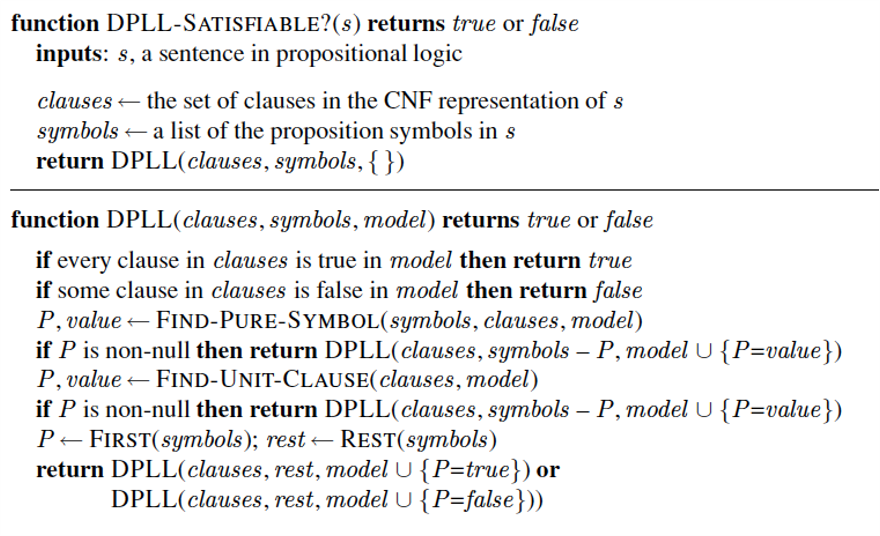
\includegraphics[width=0.9\textwidth]{immagini/DPLL.png}
\end{figure}

\subsubsection{Miglioramenti di DPLL}

DPLL è completo e termina sempre.\
Alcuni miglioramenti:
\begin{itemize}
	\item Analisi di componenti (sotto-problemi indipendenti):\ se le variabili possono essere suddivise in sotto-insiemi disgiunti (senza simboli in comune).
	\item Ordinamento di variabili e valori:\ scegliere la variabile che compare in più clausole.
	\item Backtracking intelligente e altre ottimizzazioni\dots
\end{itemize}

\subsection{Metodi locali per SAT}

Gli stati sono assegnamenti completi, l'obiettivo è un assegnamento che soddisfi tutte le clausole (un modello).\
Si parte da un assegnamento casuale e ad ogni passo si cambia il valore di un simbolo proposizionale (\textbf{\textit{flip}}).\
Gli stati sono valutati contando il numero di clausole \textbf{non soddisfatte} (meno sono meglio è) [o soddisfatte].\

Ci sono molti minimi locali per sfuggire ai quali serve introdurre perturbazioni casuali
\begin{itemize}
	\item Hill climbing con riavvio casuale
	\item Simulated Annealing
\end{itemize}
Molta sperimentazione per trovare il miglior compromesso tra il grado di ``avidità'' e casualità.\
WALK-SAT è uno degli algoritmi più semplici ed efficaci.

\subsubsection{WalkSAT}

WalkSAT ad ogni passo sceglie a caso una clausola non ancora soddisfatta, sceglie un simbolo da modificare (\textit{flip}) con probabilità \textit{p} (di solito 0,5) tra una delle due:
\begin{itemize}
	\item sceglie un simbolo a caso (\textbf{passo casuale}),
	\item sceglie quello che rende più clausole soddisfatte (\textbf{passo di ottimizzazione}).
\end{itemize}
Il passo casuale corrisponde a un \textbf{random walk} locale, quello di ottimizzazione a un tentativo di andare in salita.

Si arrende dopo un certo numero di \textit{flip} predefinito.

\begin{figure}[H]
	\centering
	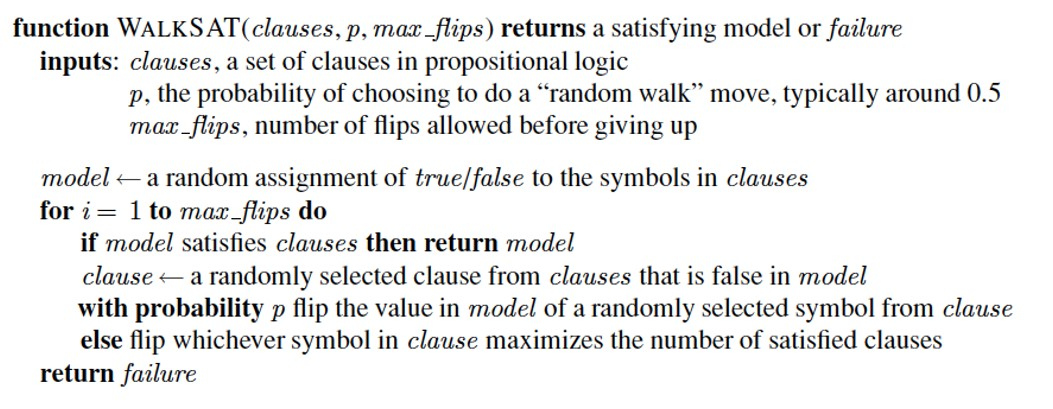
\includegraphics[width=0.9\textwidth]{immagini/WalkSAT.jpg}
\end{figure}

\subsubsection{Analisi di WalkSAT}

Se \textit{max-flips} $= \infty$ e l'insieme di clausole è soddisfacibile, prima o poi termina.\
Va bene per cercare un modello, sapendo che c'è, ma se è insoddisfacibile non termina quindi non può essere usato per verificare l'insoddisfacibilità.\

Il problema è decidibile ma l'algoritmo non è completo.

\subsubsection{Problemi SAT difficili}

Se un problema ha molte soluzioni (problema sotto-vincolato) è più probabile che WalkSAT ne trovi una in tempi brevi.\
Per esempio se ho 16 soluzioni su 32; un assegnamento ha il 50\% di probabilità di essere giusto:\ 2 passi in media!

\noindent Esempio:\ Istanza di 3SAT

\begin{center}
	($\lnot$D $\lor$ $\lnot$B $\lor$ C) $\land$ (B $\lor$ $\lnot$A $\lor$ $\lnot$C) $\land$ ($\lnot$C $\lor$ $\lnot$B $\lor$ E) $\land$ (E $\lor$ $\lnot$D $\lor$ B) $\land$ (B $\lor$ E $\lor$ $\lnot$C)
\end{center}

\noindent Quello che conta è il rapporto $m/n$, dove \textit{m} è il numero di clausole (vincoli) e \textit{n} il numero di simboli.\
In questo caso, $5/5=1$.\
Più grande il rapporto, più vincolato è il problema.\

Le regine sono facili perché il problema è sotto-vincolato.

\subsection{Inferenza come deduzione}

Un altro modo per decidere se KB $\models$ A è usare un \textbf{sistema di deduzione}; si scrive KB $\vdash$ A  (A è deducibile da KB).\
La deduzione avviene specificando delle \textbf{regole di inferenza}.

In un sistema di inferenza le regole
\begin{itemize}
	\item dovrebbero derivare \textit{solo} formule che sono conseguenza logica,
	\item dovrebbero derivare \textit{tutte} le formule che sono conseguenza logica.
\end{itemize}

\subsubsection{Correttezza e completezza}
\begin{center}
	\textbf{Correttezza}:\ Se KB $\vdash$ A allora KB $\models$ A
\end{center}
Tutto ciò che è derivabile è conseguenza logica.\ Le regole preservano la verità.
\begin{center}
	\textbf{Completezza}:\ Se KB $\models$ A allora KB $\vdash$ A
\end{center}
Tutto ciò che è conseguenza logica è ottenibile tramite il sistema deduttivo.

\subsubsection{Dimostrazione come ricerca}

\textit{Problema}:\ come decidere ad ogni passo qual è la regola di inferenza da applicare?\ \dots e a quali premesse?\ Come evitare l'esplosione combinatoria?

Si tratta di un problema di esplorazione di uno spazio di stati.\
Una \textit{procedura di dimostrazione} definisce:
\begin{itemize}
	\item la direzione della ricerca,
	\item la strategia di ricerca.
\end{itemize}

\subsubsection{Direzione della ricerca}
Nella dimostrazione di teoremi conviene procedere all'indietro.\
Con una applicazione \textit{in avanti} delle regole di inferenza non controllata:\ da A, B posso derivare A $\land$ B, A $\land$ (A $\land$ B), \dots, A $\land$ (A $\land$ (A $\land$ B)).

Meglio \textit{all'indietro}:
\begin{itemize}
	\item se si vuole dimostrare A $\land$ B, si cerchi di dimostrare A e poi B
	\item se si vuole dimostrare A $\Rightarrow$ B, si assuma A e si cerchi di dimostrare B
	      %\item \dots
\end{itemize}

\subsubsection{Strategia di ricerca}

\textit{Completezza}
\begin{itemize}
	\item Le regole della deduzione naturale sono un insieme di regole di inferenza completo (2 per ogni connettivo)
	\item Se l'algoritmo di ricerca è completo siamo a posto
\end{itemize}
\textit{Efficienza} $\rightarrow$ la complessità è alta:\ è un problema decidibile ma NP-completo.

\subsubsection{Regola di risoluzione per PROP}

Meno regole ci sono e meglio è, senza rinunciare alla completezza.\
Un'unica regola:\ la regola di risoluzione (presuppone forma a clausole).

\[
	\frac{\{P,Q\}\quad \{\lnot,R\}}{\{Q,R\}} \qquad \frac{P\lor Q\quad \lnot P \lor R}{Q \lor R}
\]

\noindent È corretta?\ Basta pensare ai modelli.\
Il motivo per cui viene preferita la notazione insiemistica è che gli eventuali duplicati si eliminano.

\subsubsection{La regola di risoluzione generale}

\[
	\frac{\{l_1,l_2,\dots, l_i, \dots, l_k\} \quad \{m_1, m_2, \dots, m_j, \dots, m_n\}}{\{l_1,l_2,\dots, l_{i-1}, l_{i+1}, \dots, l_k, m_1, m_2, \dots, m_{j-1}, m_{j+1}, \dots, m_n\}}
\]
Gli \textit{l} e \textit{m} sono \textbf{letterali}, simboli di proposizione positivi o negativi; \textit{\textbf{l}\textsubscript{i}} e \textit{\textbf{m}\textsubscript{j}} sono uguali e di segno opposto.\

\vspace{12pt}

\noindent Caso particolare:\ clausola vuota $\rightarrow$ \textit{contraddizione}.

\[
	\frac{\{P\}\quad \{\lnot P\}}{\{\ \}}
\]
\noindent La regola è sufficiente?\ È sicuro che applicando la regola in tutti i modi possibili si riesca a dedurre A quando è conseguenza logica?

\textbf{Completezza}:\ se KB $\models \alpha$ allora KB $\vdash$\textsubscript{res} $\alpha$?\ Non sempre, per esempio KB $\models$ \{A, $\lnot$A\}, ma non è vero che KB $\vdash$\textsubscript{res} \{A, $\lnot$A\}.\

Nella versione proposizionale è di aiuto il teorema di risoluzione [ground]:
\begin{center}
	KB insoddisfacibile \textit{sse} KB $\vdash$\textsubscript{res} \{ \}
\end{center}
in qualche modo si tratta di una garanzia di \textit{completezza}.\
Il teorema di refutazione offre un modo alternativo:\

\begin{center}
	KB $\models \alpha$ \textit{sse} (KB $\cup\ \{\lnot \alpha \}$) è insoddisfacibile
\end{center}

\noindent Nell'esempio:\ KB $\cup$ FC ($\lnot$(A $\lor$ $\lnot$A)) è insoddisfacibile?\ Sì, perché\dots KB $\cup$ \{A\} $\cup$ \{$\lnot$A\} $\vdash$\textsubscript{res} \{ \} in un passo.\ Quindi KB $\models$  \{A, $\lnot$A\}.

\subsubsection{Conclusioni}

\begin{itemize}
	\item Abbiamo visto come gli agenti KB che usano PROP come linguaggio di rappresentazione possono decidere se KB $\models \alpha$.
	\item Il problema è decidibile, ma intrattabile (NP) nel caso peggiore.
	\item Esistono algoritmi efficienti e completi che consentono di affrontare problemi di grosse dimensioni.
	\item I metodi locali sono particolarmente efficienti ma non completi.
\end{itemize}

